% !TEX encoding = UTF-8
% !TEX program = xelatex
\documentclass[12pt,a4paper]{article}
\usepackage[paperwidth=210mm, paperheight=297mm, left=0.75in, right=0.75in, bottom=1in, top=1in]{geometry}
\usepackage{polyglossia}
\setdefaultlanguage[babelshorthands]{italian}
\usepackage{fontspec}
\usepackage{graphicx}
\usepackage{blindtext}
\usepackage{wrapfig}

\frenchspacing
\makeindex

\begin{document}
\title{\vspace{-70pt}Hipparcos}
\author{Eleonora Lenotti}
\date{}
\maketitle
\pagestyle{empty}
\thispagestyle{empty}

% aggiungere asterischi
% cambiare nome e autore
% spostare figura
% pack

\section*{Storia}
\label{storia}
\begin{wrapfigure}{r}{0.35\textwidth}
  \vspace{-10pt}
  \begin{center}
    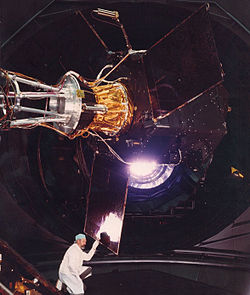
\includegraphics[width=0.30\textwidth]{satellite}
  \end{center}
  \vspace{-20pt}
\end{wrapfigure}
Hipparcos, acronimo di High Precision Parallax Collecting Satellite (Satellite per ottenere parallassi ad alta precisione), detto anche Hipparcos Space Astrometry Mission (Missione di astrometria spaziale Hipparcos), la prima missione spaziale dedicata all'astrometria, accettata nel programma scientifico dell'Agenzia Spaziale Europea ESA nel 1980.
Il progetto è stato chiamato in questo modo in onore di Ipparco.
Il satellite è stato ideato e costruito, sotto la supervisione dell'ESA, da un consorzio industriale costituito dalla Matra Marconi Space (Francia) e dall'Alenia Spazio (Italia).
Il progetto era dedicato alla misura delle parallassi stellari, cosa che permette di ricavare la distanza di una stella, e del moto proprio delle stelle. Il satellite è stato utilizzato per misurare la distanza di 2 milioni e mezzo di stelle, situate fino a 150 parsec (circa 400 anni luce) di distanza, raccolte nel Catalogo Tycho.
Il progetto iniziale del satellite fu proposto nel 1980, e fu presto approvato vista l'importanza del fornire misure di base su cui poi le teorie astrofisiche potessero basarsi. Il satellite fu lanciato da un razzo Ariane 4 il 18 agosto 1989, dalla base spaziale di Kourou, nella Guyana francese. L'obiettivo originale era di piazzarlo in un'orbita geostazionaria, ma un guasto al razzo risultò in un'orbita altamente ellittica. Nonostante questa difficoltà, quasi tutti gli obiettivi della missione furono realizzati. Il satellite è stato spento il 17 agosto 1993.

\section*{Osservazioni}
\label{osservazioni}

Il programma di lavoro era diviso in due parti: l'esperimento Hipparcos, il cui obiettivo era di misurare i parametri astro metrici di circa 120.000 stelle con una precisione da 2 a 4 milli-arcosecondi, e l'esperimento Tycho, la misura delle proprietà astrometriche e di fotometria in due colori di 400.000 stelle ad una precisione leggermente inferiore.
Il Catalogo Hipparcos finale (120.000 stelle con risoluzione di 1 milliarcsec) e il Catalogo Tycho finale (più di un milione di stelle con risoluzione di 20--30 milliarcsec e fotometria a 2 colori) furono completati nell'agosto del 1996, e pubblicati dall'ESA nel giugno del 1997.
I dati dei due cataloghi sono stati utilizzati per realizzare il Millennium Star Atlas (Atlante Stellare del Millennio): un atlante di tutto il cielo, comprendente un milione di stelle fino alla magnitudine 11 dai dati Hipparcos, più circa 10.000 oggetti non stellari.
Sebbene poco appariscente, il lavoro di Hipparcos è di importanza fondamentale: senza misure accurate di posizione e soprattutto di distanza non si può fare astrofisica. La parallasse stellare è l'unico metodo diretto per misurare le distanze delle stelle: tutti gli altri, come le candele standard, sono metodi indiretti e incerti che si basano sulla parallasse per essere calibrati correttamente.
C'è da dire che è stato riscontrato un errore di tracciamento delle stelle in Hipparcos (dovuto a leggere variazioni di temperatura), per cui Floor van Leeuwen, dell'osservatorio di Cambridge, ha compiuto un lavoro decennale di ricalcolo delle posizioni stellari. Il risultato è il catalogo di stelle più accurato che esista, che si intitola ``Hipparcos. The new reduction of the raw data.''.

\end{document}